\documentclass[14pt]{report}
\usepackage[T2A]{fontenc}
\usepackage[utf8]{inputenc}
\usepackage[english,russian]{babel}
\usepackage{listings}
\pagestyle{plain}
\usepackage{geometry}
\usepackage{amssymb}
\usepackage{amsmath}
\usepackage{indentfirst}
\usepackage[14pt]{extsizes}
\geometry{left=2cm}
\geometry{right=1.5cm}
\geometry{top=1cm}
\geometry{bottom=2cm}
\usepackage{pgfplots}
\usepackage{filecontents}
\usepackage{graphicx}
\DeclareGraphicsExtensions{.png}
\graphicspath{{images/}}
\usetikzlibrary{datavisualization}
\usetikzlibrary{datavisualization.formats.functions}
\frenchspacing
\usepackage{tocloft}

\renewcommand\cftchapdotsep{\cftdot}
\renewcommand\cftsecdotsep{\cftdot}
\renewcommand{\cftchapleader}{\cftdotfill{\cftchapdotsep}}

% Для листинга кода:
\lstset{ %
language=python,                 % выбор языка для подсветки
basicstyle=\small\sffamily, % размер и начертание шрифта для подсветки кода
numbers=left,               % где поставить нумерацию строк (слева\справа)
numberstyle=\tiny,           % размер шрифта для номеров строк
stepnumber=1,                   % размер шага между двумя номерами строк
numbersep=5pt,                % как далеко отстоят номера строк от подсвечиваемого кода
showspaces=false,            % показывать или нет пробелы специальными отступами
showstringspaces=false,      % показывать или нет пробелы в строках
showtabs=false,             % показывать или нет табуляцию в строках
frame=single,              % рисовать рамку вокруг кода
tabsize=4,                 % размер табуляции по умолчанию равен 2 пробелам
captionpos=t,              % позиция заголовка вверху [t] или внизу [b]
breaklines=true,           % автоматически переносить строки (да\нет)
breakatwhitespace=false, % переносить строки только если есть пробел
escapeinside={\#*}{*)}   % если нужно добавить комментарии в коде
}

% Для измененных титулов глав:
\usepackage{titlesec, blindtext, color} % подключаем нужные пакеты
\definecolor{gray75}{gray}{0.75} % определяем цвет
\newcommand{\hsp}{\hspace{20pt}} % длина линии в 20pt
% titleformat определяет стиль
\titleformat{\chapter}[hang]{\Huge\bfseries}{\thechapter\hsp\textcolor{gray75}{|}\hsp}{0pt}{\Huge\bfseries}


\begin{filecontents}{LevM.dat}
0 2.58e-06
50 0.00032896
100 0.00067026
150 0.00100624
200 0.00176384
250 0.00273216
300 0.00392608
350 0.00531646
400 0.00692414
450 0.0087609
500 0.0108672
550 0.0131632
600 0.0156044
650 0.0182917
700 0.0212066
750 0.0244535
800 0.0281559
850 0.0314529
900 0.0354612
950 0.0392116
1000 0.0433937
\end{filecontents}

\begin{filecontents}{DamLevM.dat}
0	5.4e-07
50	0.00017596
100	0.00071314
150	0.00159782
200	0.0028283
250	0.00448456
300	0.00650698
350	0.00876206
400	0.0114267
450	0.0145368
500	0.0179466
550	0.0217669
600	0.0257943
650	0.0303514
700	0.0356014
750	0.0403816
800	0.0460019
850	0.0519328
900	0.0581385
950	0.0649824
1000	0.0723375
\end{filecontents}

\begin{filecontents}{DamLevM2.dat}
0 2.2e-06
1 1.9e-06
2 2.7e-06
3 3.6e-06
4 4.7e-06
5 6.4e-06
6 8.2e-06
7 1.11e-05
8 1.38e-05
9 1.69e-05
10 2.1e-05
\end{filecontents}


\begin{filecontents}{DamLevR.dat}
0	1.9e-06
1	3.6e-06
2	1.04e-05
3	3.97e-05
4	0.0001972
5	0.0008738
6	0.0030926
7	0.0101053
8	0.0550824
9	0.303918
10	1.69359
\end{filecontents}


\begin{document}
\begin{titlepage}
	\centering
	{\scshape\LARGE МГТУ им. Баумана \par}
	\vspace{3cm}
	{\scshape\Large Лабораторная работа №1\par}
	\vspace{0.5cm}
	{\scshape\Large По курсу: "Анализ алгоритмов"\par}
	\vspace{1.5cm}
	{\huge\bfseries Расстояние Левенштейна\par}
	\vspace{2cm}
	\Large Работу выполнила: Овчинникова Анастасия, ИУ7-55Б\par
	\vspace{0.5cm}
	\LargeПреподаватели:  Волкова Л.Л., Строганов Ю.В.\par

	\vfill
	\large \textit {Москва, 2019} \par
\end{titlepage}

\tableofcontents

\newpage

\chapter*{Введение}
\addcontentsline{toc}{chapter}{Введение}

\textbf{Расстояние Левенштейна (редакторское расстояние)} - это минимальное количество операций (вставки одного символа, удаления одного символа и замены одного символа на другой), которое необходимо для преобразования строки s1 в строку s2.
Расстояние Левенштейна широко используется в теории информации, биоинформатике и компьютерной лингвистике:
\begin{itemize}
	\item для исправления ошибок в слове (в поисковых системах, базах данных, при вводе текста, при автоматическом распознавании отсканированного текста или речи);
	\item для сравнения текстовых файлов утилитой diff и ей подобными;
	\item в биоинформатике для сравнения генов, хромосом и белков.
\end{itemize}

Расстояние Дамерау-Левенштейна - это расстояние Левенштейна, расширенное перестановкой соседних символов.

Целью данной работы является изучение метода динамического программирования на материале алгоритмов Левенштейна и Дамерау-Левенштейна.
Задачи данной лабораторной:
\begin{itemize}
	\item изучение алгоритмов Левенштейна и Дамерау-Левенштейна нахождения расстояния между строками;
	\item применение метода динамического программирования для матричной реализации указанных алгоритмов;
	\item получение практических навыков реализации указанных алгоритмов:  двух алгоритмов в матричной и в рекурсивной версиях;
	\item сравнительный анализ линейной и рекурсивной реализаций выбранного алгоритма определения расстояния между строками по затрачиваемым ресурсам (времени и памяти);
	\item экспериментальное подтверждение различий во временнóй эффективности рекурсивной и нерекурсивной реализаций выбранного алгоритма определения расстояния между строками при помощи разработанного программного обеспечения на материале замеров процессорного времени выполнения реализации на варьирующихся длинах строк;
	\item описание и обоснование полученных результатов в отчете о выполненной лабораторной работе, выполненного как расчётно-пояснительная записка к работе.
\end{itemize}

\chapter*{Аналитическая часть}
\addcontentsline{toc}{chapter}{Аналитическая часть}

Задача по нахождению расстояния Левенштейна заключается в поиске минимального количества операций вставки одного символа, удаления одного символа и замены одного символа на другой, необходимых для превращения одной строки в другую.

Вводятся следующие разрешенные редакторские операции над строкой:
\begin{itemize}
	\item I (англ. insert) - вставка;
	\item D (англ. delete) - удаление;
	\item R (англ. replace) - замена;
	\item M (англ. match) - совпадение.
\end{itemize}

При нахождении расстояния Дамерау-Левенштейна добавляется еще одна операция:
\begin{itemize}
	\item T (англ. transpose) - транспозиция (перестановка соседних символов).
\end{itemize}

Пусть $S_{1}$ и $S_{2}$ — две строки (длиной M и N соответственно) над некоторым алфавитом, тогда редакционное расстояние можно подсчитать по следующей рекуррентной формуле:
\begin{displaymath}
D(i,j) = \left\{ \begin{array}{ll}
 0, & \textrm{$i = 0, j = 0$}\\
 i, & \textrm{$j = 0, i > 0$}\\
 j, & \textrm{$i = 0, j > 0$}\\
min(\\
D(i,j-1)+1,\\
D(i-1, j) +1, &\textrm{$j>0, i>0$}\\
D(i-1, j-1) + m(S_{1}[i], S_{2}[j])\\
),
  \end{array} \right.
\end{displaymath}

где $m(a,b)$ равна нулю, если $a=b$ и единице в противном случае; $min\{\,a,b,c\}$ возвращает наименьший из аргументов.

Расстояние Дамерау-Левенштейна вычисляется по следующей рекуррентной формуле:

\[ D(i, j) =  \left\{
\begin{aligned}
&0, && i = 0, j = 0\\
 &i, && i > 0, j = 0\\
 &j, && i = 0, j > 0\\
 &min \left\{
\begin{aligned}
 &D(i, j - 1) + 1,\\
			 &D(i - 1, j) + 1,\\
			 &D(i - 1, j - 1) + m(S_{1}[i], S_{2}[i]), \\
			 &D(i - 2, j - 2) + m(S_{1}[i], S_{2}[i]),\\
	 \end{aligned} \right.
	 &&
\begin{aligned}
 &, \text{ если } i, j > 0 \\
			 & \text{ и } S_{1}[i] = S_{2}[j - 1] \\
			 & \text{ и } S_{1}[i - 1] =  S_{2}[j] \\
	 \end{aligned} \\
	 &min \left\{
	 \begin{aligned}
			 &D(i, j - 1) + 1,\\
			 &D(i - 1, j) + 1, \\
			 &D(i - 1, j - 1) + m(S_{1}[i], S_{2}[i]),\\
	 \end{aligned} \right.  &&, \text{иначе}
\end{aligned} \right.
\]

%\begin{displaymath}
%D(i,j) = \left\{ \begin{array}{ll}
% 0, & \textrm{$i = 0, j = 0$}\\
% i, & \textrm{$j = 0, i > 0$}\\
% j, & \textrm{$i = 0, j > 0$}\\
%min(\\
%D(i,j-1)+1,\\
%D(i-1, j) +1, &\textrm{$j>0, i>0$}\\
%D(i-1, j-1) + m(S_{1}[i], S_{2}[j])\\
%)
%  \end{array} \right.
%\end{displaymath}

%\textrm{if $i,j>1$ and $a_{i} = b_{j-1},a_{i-1}=b_{j} $}\\
% D(i-2, j-2) + 1


Оба алгоритма можно реализовать с помощью таблицы (матрично).

Пусть имеются строки $s_{1}$ = 'скат' и $s_{2}$ = 'кот'. Необходимо вычислить редакторское расстояние между строками s1 и s2.

Для вычисления расстояния составляется следующая таблица (символ $\varnothing$ обозначает пустую строку):

\begin{tabular}{ | c || c | c | c | c | }
\hline
    & $\varnothing$ & к & о & т \\ \hline \hline
	$\varnothing$ &  &  &  &  \\ \hline
	с &  &  &  &  \\ \hline
  к &  &  &  &  \\ \hline
  а &  &  &  &  \\ \hline
  т &  &  &  &  \\ \hline
\end{tabular}

При заполнении таблицы для каждой из операций (вставка, удаление, замена, совпадение, транспозиция) нужно учитывать штрафы:
\begin{itemize}
	\item Вставка - штраф 1;
	\item Удаление - штраф;
	\item Замена - штраф 1;
	\item Транспозиция - штраф 1;
	\item Совпадение - штраф 0.
\end{itemize}

В каждую клетку заносится значение $D(s_{1}[i], s_{2}[j])$, где $i >= 0, j >= 0$ номера текущей строки и текущего столбца соответственно (нумерация начинается с 0).

На следующем шаге заполняются тривиальные случаи: нулевой столбец и нулевая строка (строки не являются частью таблицы).

\begin{tabular}{ | c || c | c | c | c | }
\hline
    & $\varnothing$ & к & о & т \\ \hline \hline
	$\varnothing$ & 0 & 1 & 2 & 3 \\ \hline
	с & 1 &  &  &  \\ \hline
  к & 2 &  &  &  \\ \hline
  а & 3 &  &  &  \\ \hline
  т & 4 &  &  &  \\ \hline
\end{tabular}

Для $i > 0, j > 0$ выбирается минимальный ход из трех возможных:

\begin{tabular}{ | c | c | }
\hline
  x  & y  \\ \hline
	z & $min(y + 1, z + 1, x + fine)$ \\ \hline
\end{tabular}


\begin{equation*}
\text{где }fine =
 \begin{cases}
	 1 &\text{, если $s_{1}[i] = s_{2}[j]$}\\
   0 &\text{, иначе.}
 \end{cases}
\end{equation*}

Так, для $i = 1, j = 1$:

\begin{tabular}{ | c | c | }
\hline
  x =0   & y = 1  \\ \hline
	z = 1 & $min(y + 1 = 2, z + 1 = 2, x + fine = x + 0 = 1)$ \\ \hline
\end{tabular}

Заносим в таблицу полученное значение:

\begin{tabular}{ | c || c | c | c | c | }
\hline
    & $\varnothing$ & к & о & т \\ \hline \hline
	$\varnothing$ & 0 & 1 & 2 & 3 \\ \hline
	с & 1 & 1 &  &  \\ \hline
  к & 2 &  &  &  \\ \hline
  а & 3 &  &  &  \\ \hline
  т & 4 &  &  &  \\ \hline
\end{tabular}

Проделав данную операцию для всех клеток, получим:

\begin{tabular}{ | c || c | c | c | c | }
\hline
    & $\varnothing$ & к & о & т \\ \hline \hline
	$\varnothing$ & 0 & 1 & 2 & 3 \\ \hline
	с & 1 & 1 & 2 & 3 \\ \hline
  к & 2 & 1 & 2 & 3 \\ \hline
  а & 3 & 2 & 2 & 3 \\ \hline
  т & 4 & 3 & 3 & {\bf2} \\ \hline
\end{tabular}

Искомое редакторское расстояние выделено жирным шрифтом.

При нахождении расстояния Дамерау-Левенштейна матричным способом при вычислении нетривиальных случаев необходимо учитывать еще один возможный ход:

\begin{tabular}{ | c | c | c |}
\cline{1-1}
  g \\ \cline{1-1} \cline{1-2} \cline{1-3}
  \multicolumn{1}{c|}{} & x & y \\ \cline{2-1} \cline{3-1}
	\multicolumn{1}{c|}{} & z & $min(y + 1, z + 1, x + fine, g + 1)$ \\ \cline{2-1} \cline{3-1}
\end{tabular}


\begin{equation*}
\text {$g$ учитывается, только если}
 \begin{cases}
	 len(s_{1}) >= 2 \\
	 len(s_{2}) >= 2 \\
	 s_{1}[i] = s_{2}[j-1] \\
   s_{2}[j] = s_{1}[i-1]
 \end{cases}
\end{equation*}

где $len(s)$ - длина строки $s$.

\chapter*{Конструкторская часть}
\addcontentsline{toc}{chapter}{Конструкторская часть}

\section*{Требования к входным данным}
\addcontentsline{toc}{section}{Требования к входным данным}
\begin{enumerate}
	\item На вход программе подается две строки.
	\item Строки могут быть пустыми.
	\item Строчные и прописные буквы считаются разными.
\end{enumerate}

\section*{Требования к программе}
\addcontentsline{toc}{section}{Требования к программе}
Программа представляет собой консольное приложение с меню для выбора пользователем необходимого действия.
Меню содержит следующие пункты:
\begin{itemize}
	\item "1 - расстояние Левенштейна матрично";
	\item "2 - расстояние Левенштейна рекурсивно";
	\item "3 - расстояние Дамерау-Левенштейна матрично";
	\item "4 - расстояние Дамерау-Левенштейна рекурсивно";
	\item "5 - все сразу (1-4)";
	\item "6 - временной анализ";
	\item "7 - тесты".
\end{itemize}

Для выбора соответствующих пунктов меню пользователь вводит соответствующую цифру (1-7). При вводе любого другого символа программа должна корректно завершаться.

При выборе пунктов 1-5 программа попросит пользователя ввести две строки. Ввод пустых строк считается корректым, программа при этом не должна аварийно завершаться.

\section*{Схемы алгоритмов}
\addcontentsline{toc}{section}{Схемы алгоритмов}

Схема матричного алгоритма для вычисления расстояния Левенштейна представлена на рисунке 1. Схема матричного алгоритма для вычисления расстояния Дамерау-Левенштейна представлена на рисунке 2.
Схема рекурсивного алгоритма для вычисления расстояния Левенштейна представлена на рисунке 3. Схема рекурсивного алгоритма для вычисления расстояния Дамерау-Левенштейна представлена на рисунке 4.

\begin{figure}
\center{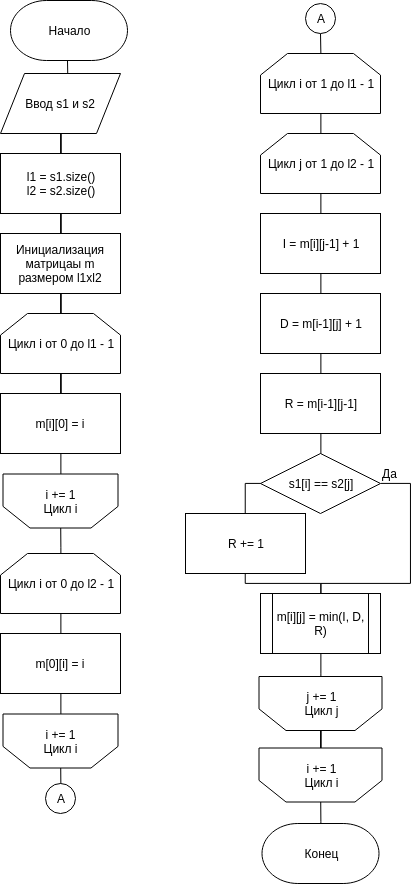
\includegraphics[height=20cm]{LevMatr}}
\caption{Матричный алгоритм для вычисления расстояния Левенштейна}
\label{fig:image}
\end{figure}

\begin{figure}
\center{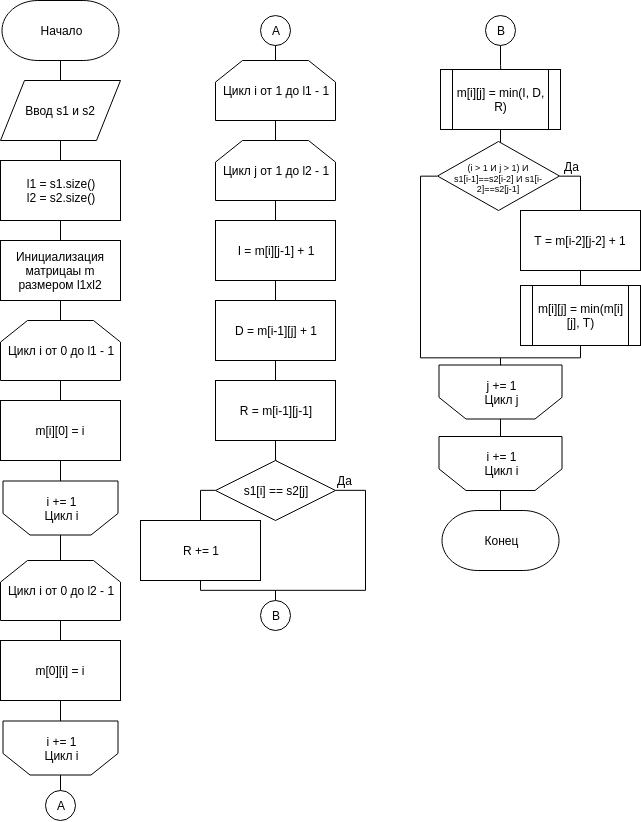
\includegraphics[height=20cm]{DamLevMatr}}
\caption{Матричный алгоритм для вычисления расстояния Дамерау-Левенштейна}
\label{fig:image}
\end{figure}

\begin{figure}
\center{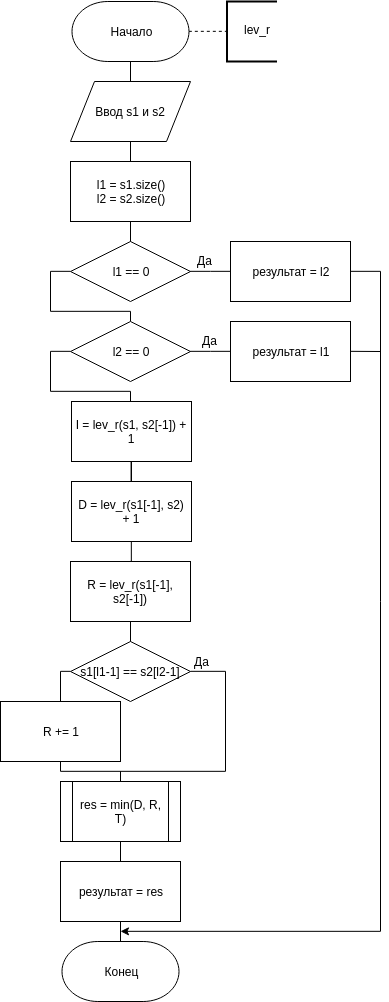
\includegraphics[height=20cm]{LevRec}}
\caption{Рекурсивный алгоритм для вычисления расстояния Левенштейна}
\label{fig:image}
\end{figure}

\begin{figure}
\center{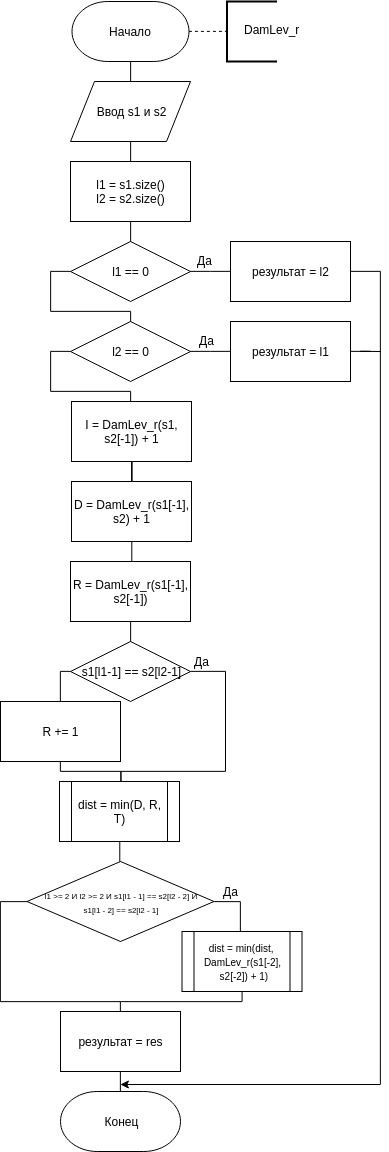
\includegraphics[height=20cm]{DamLevRec}}
\caption{Рекурсивный алгоритм для вычисления расстояния Дамерау-Левенштейна}
\label{fig:image}
\end{figure}


\section*{Выбор языка программирования}
\addcontentsline{toc}{section}{Выбор языка программирования}

В качестве языка программирования для реализации программы был выбран язык C++ и фреймворк Qt, потому что:
\begin{itemize}
	\item язык C++ имеет высокую вычислительную производительность;
	\item язык C++ поддерживает различные стили программирования;
	\item стандартные строки C++ (std::string) не поддерживают юникод, поэтому вместо std::string были использованы строки Qt (QString);
	\item в Qt существует удобный инструмент для тестирования - QtTest - который позволяет собирать тесты в группы, собирать результаты выполнения тестов, а также уменьшить дублирование кода при схожих объектах тестирования.
\end{itemize}

Для замеров времени использовалась функция clock() модуля ctime. Эта функция возвращает количество временных тактов, прошедших с начала запуска программы. С помощью макроса CLOCKS\_PER\_SEC можно узнать количество пройденных тактов за 1 секунду.

\section*{Сведения о модулях программы}
\addcontentsline{toc}{section}{Сведения о модулях программы}

Программа состоит из следующих файлов:
\begin{itemize}
	\item devenshteindistance.h, devenshteindistance.cpp - заголовочный файл и файл, в котором расположена реализация алгоритмов;
	\item main.cpp - главный файл программы, в котором расположена реализация меню;
	\item testdistance.h, testdistance.cpp - файл и заголовочный файл, в котором расположена реализация тестов.
\end{itemize}


\begin{lstlisting}[label=some-code,caption=Функция для нахождения расстояния Левенштейна матрично]
int LevenshteinDistance::levenshteinDistance_m(QString s1, QString s2)
{
    int l1 = s1.size() + 1;
    int l2 = s2.size() + 1;

    int * matrix = (int*) calloc(l1 * l2, sizeof (int));

    for (int i = 0; i < l1; ++i)
    {
        for (int j = 0; j < l2; ++j)
        {
            matrix[i*l2 + j] = 0;
        }
    }

    for (int i = 1; i < l2; ++i)
        matrix[i] = i;
    for (int i = 1; i < l1; ++i)
        matrix[i*l2] = i;

    for (int i = 1; i < l1; ++i)
    {
        for (int j = 1; j < l2; ++j)
        {
            int r1 = matrix[(i - 1)*l2 + j] + 1;
            int r2 = matrix[i*l2 + (j - 1)] + 1;

            int fine = 1;
            if (s1.at(i - 1) == s2.at(j - 1))
            {
                fine = 0;
            }
            int r3 = matrix[(i - 1)*l2 + (j - 1)] + fine;
            matrix[i*l2 + j] = myMin(r1, r2, r3);
        }
    }
    if (printMatrixFlag)
    {
        cout << "Matrix: " << endl;
        printMatrix(matrix, l1, l2);
    }
    int d = matrix[(l1 - 1)*l2 + (l2 - 1)];
    free(matrix);
    return d;
}
\end{lstlisting}

\begin{lstlisting}[label=some-code,caption=Функция для нахождения расстояния Левенштейна рекурсивно]
int LevenshteinDistance::levenshteinDistance_r(QString s1, QString s2)
{
    if (s1.size() == 0 && s2.size() == 0)
        return 0;
    if (s1.size() == 0)
        return s2.size();
    if (s2.size() == 0)
        return s1.size();

    QString newS1 = s1.left(s1.size() - 1);
    QString newS2 = s2.left(s2.size() - 1);
    int r1 = levenshteinDistance_r(newS1, s2) + 1;
    int r2 = levenshteinDistance_r(s1, newS2) + 1;
    int r3 = levenshteinDistance_r(newS1, newS2);
    if (s1.at(s1.size() - 1) != s2.at(s2.size() - 1))
        r3 += 1;
    int distance = myMin(r1, r2, r3);
    return distance;
}
\end{lstlisting}

\begin{lstlisting}[label=some-code,caption=Функция для нахождения расстояния Дамерау-Левенштейна матрично]
int LevenshteinDistance::damerauLevenshteinDistance_m(QString s1, QString s2)
{
    int l1 = s1.size() + 1;
    int l2 = s2.size() + 1;

    int * matrix = (int*) calloc(l1 * l2, sizeof (int));

    for (int i = 0; i < l1; ++i)
    {
        for (int j = 0; j < l2; ++j)
        {
            matrix[i*l2 + j] = 0;
        }
    }

    for (int i = 1; i < l2; ++i)
        matrix[i] = i;
    for (int i = 1; i < l1; ++i)
        matrix[i*l2] = i;

    for (int i = 1; i < l1; ++i)
    {
        for (int j = 1; j < l2; ++j)
        {
            int r1 = matrix[(i - 1)*l2 + j] + 1;
            int r2 = matrix[i*l2 + (j - 1)] + 1;

            int fine = 1;
            if (s1.at(i - 1) == s2.at(j - 1))
            {
                fine = 0;
            }
            int r3 = matrix[(i - 1)*l2 + (j - 1)] + fine;
            int distance = myMin(r1, r2, r3);

            if (i > 1 && j > 1)
            {
                if (s1.at(i-1) == s2.at(j-2) && s2.at(j-1) == s1.at(i-2))
                    distance = min(distance, matrix[(i-2)*l2 + (j-2)] + 1);
            }
            matrix[i*l2 + j] = distance;
        }
    }
    if (printMatrixFlag)
    {
        cout << "Matrix: " << endl;
        printMatrix(matrix, l1, l2);
    }
    int d = matrix[(l1 - 1)*l2 + (l2 - 1)];
    free(matrix);
    return d;
}
\end{lstlisting}

\begin{lstlisting}[label=some-code,caption=Функция для нахождения расстояния Дамерау-Левенштейна рекурсивно]
int LevenshteinDistance::damerauLevenshteinDistance_r(QString s1, QString s2)
{
    if (s1.size() == 0 && s2.size() == 0)
        return 0;
    if (s1.size() == 0)
        return s2.size();
    if (s2.size() == 0)
        return s1.size();

    int l1 = s1.size();
    int l2 = s2.size();

    QString newS1 = s1.left(l1 - 1);
    QString newS2 = s2.left(l2 - 1);
    int r1 = levenshteinDistance_r(newS1, s2) + 1;
    int r2 = levenshteinDistance_r(s1, newS2) + 1;
    int r3 = levenshteinDistance_r(newS1, newS2);
    if (s1.at(l1 - 1) != s2.at(l2 - 1))
        r3 += 1;
    int distance = myMin(r1, r2, r3);

    if (l1 >= 2 && l2 >= 2 && s1.at(l1 - 1) == s2.at(l2 - 2) &&
            s1.at(l1 - 2) == s2.at(l2 - 1))
    {
        newS1 = s1.left(l1 - 2);
        newS2 = s2.left(l2 - 2);
        distance = min(distance, damerauLevenshteinDistance_r(newS1, newS2) + 1);
    }

    return distance;
}
\end{lstlisting}

\section*{Тесты}
\addcontentsline{toc}{section}{Тесты}

Тестирование проводилось с помощью модуля QtTest.
Для этого был написал класс  {\bf TestDistance}, который тестирует написанные алгоритмы. Тестирование алгоритмов проводилось в три шага.

Сначала каждый из алгоритмов тестировался оттельно на общем для всех четырех алгоритмов наборе тестов. Набор тестов приведен в листинге 5.
Затем проводились тесты, специфичные для каждого алгоритма (для каждой пары алгоритмов). Набор тестов приведен в листинге 6.
После этого сравнивались результаты работы двух функций: функция нахождения расстояния Левенштейна матрично с функцией расстояния Левенштейна рекурсивно, функция нахождения расстояния Дамерау-Левенштейна матрично с функцией нахождения расстояния Дамерау-Левенштейна рекурсивно. Набор тестов приведен в листинге 7. При этом использоваслся генератор случайных строк. Он приведен в листинге 8.

\begin{lstlisting}[label=some-code,caption=Общие тесты ]
void TestDistance::testEmptyString()
{
    for (int i = 0; i < methodsToTest; ++i)
    {
        QVERIFY((testObj.*methodsPtr[i])("", "") == 0);
        QVERIFY((testObj.*methodsPtr[i])("1", "") == 1);
        QVERIFY((testObj.*methodsPtr[i])("12", "") == 2);
        QVERIFY((testObj.*methodsPtr[i])("", "123456789") == 9);
    }
}

void TestDistance::testSameStrings()
{
    for (int i = 0; i < methodsToTest; ++i)
    {
        QVERIFY((testObj.*methodsPtr[i])("abc", "abc") == 0);
        QVERIFY((testObj.*methodsPtr[i])("ABC", "ABC") == 0);
        QVERIFY((testObj.*methodsPtr[i])("", "") == 0);
        QVERIFY((testObj.*methodsPtr[i])("a", "a") == 0);
    }
}

void TestDistance::testDifferentStrings()
{
    for (int i = 0; i < methodsToTest; ++i)
    {
        QVERIFY((testObj.*methodsPtr[i])("a", "") == 1);
        QVERIFY((testObj.*methodsPtr[i])("", "1") == 1);
        QVERIFY((testObj.*methodsPtr[i])("b", "c") == 1);
        QVERIFY((testObj.*methodsPtr[i])("bc", "b") == 1);
        QVERIFY((testObj.*methodsPtr[i])("bc", "c") == 1);
        QVERIFY((testObj.*methodsPtr[i])("ab", "cd") == 2);
        QVERIFY((testObj.*methodsPtr[i])("ab", "AB") == 2);
        QVERIFY((testObj.*methodsPtr[i])("Cd", "cd") == 1);

        QVERIFY((testObj.*methodsPtr[i])("skat", "kot") == 2);
        QVERIFY((testObj.*methodsPtr[i])("skat", "kat") == 1);
        QVERIFY((testObj.*methodsPtr[i])("skatskat", "skat") == 4);
        QVERIFY((testObj.*methodsPtr[i])("SKAT", "skat") == 4);
        QVERIFY((testObj.*methodsPtr[i])("SkAt", "skat") == 2);
    }
}
\end{lstlisting}

\begin{lstlisting}[label=some-code,caption=специфичные тесты ]
void TestDistance::test_levenshteinDistance_r()
{
    QVERIFY(testObj.levenshteinDistance_r("ac", "ca") == 2);
    QVERIFY(testObj.levenshteinDistance_r("abc", "cba") == 2);
}

void TestDistance::test_damerauLevenshteinDistance_m()
{
    QVERIFY(testObj.damerauLevenshteinDistance_m("ac", "ca") == 1);
    QVERIFY(testObj.damerauLevenshteinDistance_m("abc", "cba") == 2);
}
\end{lstlisting}

\begin{lstlisting}[label=some-code,caption=сравнение результатов работы двух алгоритмов ]
void TestDistance::testPairsEmpty()
{
    for (int i = 0; i < testsPerPair; ++i)
    {
        QString s1 = "";
        QString s2 = randomString(i);
        QVERIFY(testObj.levenshteinDistance_m(s1, s2) == testObj.levenshteinDistance_r(s1, s2));
        QVERIFY(testObj.levenshteinDistance_m(s2, s1) == testObj.levenshteinDistance_r(s2, s1));
    }
}

void TestDistance::testPairEqualLen()
{
    for (int i = 0; i < testsPerPair; ++i)
    {
        QString s1 = randomString(i);
        QString s2 = randomString(i);
        QVERIFY(testObj.levenshteinDistance_m(s1, s2) == testObj.levenshteinDistance_r(s1, s2));
        QVERIFY(testObj.levenshteinDistance_m(s2, s1) == testObj.levenshteinDistance_r(s2, s1));
    }
}

void TestDistance::testPairDifferentLen()
{
    for (int i = 0; i < testsPerPair; ++i)
    {
        int l1 = 1 + rand() % 10;
        int l2 = 1 + rand() % 10;
        QString s1 = randomString(l1);
        QString s2 = randomString(l2);
        QVERIFY(testObj.levenshteinDistance_m(s1, s2) == testObj.levenshteinDistance_r(s1, s2));
        QVERIFY(testObj.levenshteinDistance_m(s2, s1) == testObj.levenshteinDistance_r(s2, s1));
    }
}
\end{lstlisting}

\begin{lstlisting}[label=some-code,caption=Генератор случайных строк ]
QString TestDistance::randomString(int size)
{
    string symbols = "abcdefghigklmnopqrstuvwxyzABCDEFGHIGKLMNOPQRSTUVWXYZ1234567890";
    int symbolsSize = symbols.size();
    QString res = "";
    for (int i = 0; i < size; ++i)
    {
        res += symbols.at(rand() % (symbolsSize - 1));
    }
    return res;
}
\end{lstlisting}

Все написанные тесты были пройдены.

\chapter*{Исследовательская часть}
\addcontentsline{toc}{chapter}{Исследовательская часть}

\section*{Постановка эксперимента}
\addcontentsline{toc}{section}{Постановка эксперимента}

В рамках данной работы были проведены следующие эксперименты.
\begin{enumerate}
	\item Сравнение по времени матричных алгоритмов для вычисления расстояний Левенштейна и Дамерау-Левенштейна. Сравнение проводилось для строк длиной от 1 до 1000 с шагом 50. Каждый эксперимент проводился 100 раз.
	\item Сравнение по времени рекурсивного и итеративного алгоритмов для вычисления расстояния Дамерау-Левенштейна. Сравнение проводилось для строк длиной от 1 до 10 с шагом 1. Каждый эксперимент проводился 10 раз.
\end{enumerate}

Измерения проводились на компьютере HP Pavilion Notebook на базе Intel Core i5-7200U, 2.50 Гц с 6 Гб оперативной памяти под управлением операционной системы Linux Mint.

\section*{Сравнительный анализ на материале экспериментальных данных}
\addcontentsline{toc}{section}{Сравнительный анализ на материале экспериментальных данных}

Результаты замеров времени для сравнения времени работы матричных алгоритмов для вычисления расстояний Левенштейна и Дамерау-Левенштейна приведены в таблице 1. Зависимость времени работы матричных алгоритмов для вычисления рассояния Левенштейна и Дамерау-Левенштейна от длины входных строк представлена и на рисунке 5.

Условные обозначения в таблицах и на графиках:
\begin{itemize}
	\item Lev(M) - время работы матричного алгоритма для вычисления расстояния Левенштейна в секундах;
	\item DamLev(M) - время работы матричного алгоритма для вычисления расстояния Дамерау-Левенштейна в секундах;
	\item Lev(R) - время работы рекурсивного алгоритма для вычисления расстояния Левенштейна в секундах;
	\item DamLev(R) - время работы рекурсивного алгоритма для вычисления расстояния Дамерау-Левенштейна в секундах.
\end{itemize}

\begin{table}
	\caption{Сравнение времени работы матричных алгоритмов для вычисления расстояний Левенштейна и Дамерау-Левенштейна}
	%\begin{center}
		\begin{tabular}{|c | c | c |}
	 	\hline
		Длина строки & Lev(M), с & DamLev(M), с \\ [0.5ex]
	 	\hline\hline
		0 & 2.58e-06 & 5.4e-07 \\
		\hline
		50 & 0.00032896 & 0.00017596 \\
		\hline
		100 & 0.00067026 & 0.00071314 \\
		\hline
		150 & 0.00100624 & 0.00159782 \\
		\hline
		200 & 0.00176384 & 0.0028283 \\
		\hline
		250 & 0.00273216 & 0.00448456 \\
		\hline
		300 & 0.00392608 & 0.00650698 \\
		\hline
		350 & 0.00531646 & 0.00876206 \\
		\hline
		400 & 0.00692414 & 0.0114267 \\
		\hline
		450 & 0.0087609 & 0.0145368 \\
		\hline
		500 & 0.0108672 & 0.0179466 \\
		\hline
		550 & 0.0131632 & 0.0217669 \\
		\hline
		600 & 0.0156044 & 0.0257943 \\
		\hline
		650 & 0.0182917 & 0.0303514 \\
		\hline
		700 & 0.0212066 & 0.0356014 \\
		\hline
		750 & 0.0244535 & 0.0403816 \\
		\hline
		800 & 0.0281559 & 0.0460019 \\
		\hline
		850 & 0.0314529 & 0.0519328 \\
		\hline
		900 & 0.0354612 & 0.0581385 \\
		\hline
		950 & 0.0392116 & 0.0649824 \\
		\hline
		1000 & 0.0433937 & 0.0723375 \\
		\hline
		\end{tabular}
	%\end{center}
\end{table}

\begin{figure}
	\caption{Сравнение работы матричных алгоритмов для вычисления расстояния Левенштейна и Дамерау-Левенштейна}
	\begin{tikzpicture}
	\begin{axis}[
	    	axis lines = left,
	    	xlabel = {длина, символы},
	    	ylabel = {время, с},
		legend pos=north west,
		ymajorgrids=true
	]
	\addplot[color=blue, mark=square] table[x index=0, y index=1] {LevM.dat};
	\addplot[color=green, mark=square] table[x index=0, y index=1] {DamLevM.dat};
	\addlegendentry{LevM}
	\addlegendentry{DamLevM}
	\end{axis}
	\end{tikzpicture}
\end{figure}

Результаты сравнения по времени рекурсивного и итеративного алгоритмов для вычисления расстояния Дамерау-Левенштейна приведены в таблице 2 и на рисунке 6.

Замеры времени для более длинных строк не проводились, так как время работы рекурсивного алгоритма увеличивается экспоненциально, пропорционально количеству рекурсивных вызовов (максимальная глубина рекурсии равна длине самого длинного слова).

При увеличении длинны входных строк становится видна очень сильная разница по времени выполнения между рекурсивным и матричным алгоритмами. Уже при длине строки в 10 символов матричная реализация оказывается на порядок быстрее.

\begin{table}
	\caption{Сравнение времени выполнения рекурсивного и итеративного алгоритмов для вычисления расстояния Дамерау-Левенштейна}
	%\begin{center}
		\begin{tabular}{|c | c | c |}
	 	\hline
		Длина строки & DamLev(M), с & DamLev(R), с \\ [0.5ex]
	 	\hline\hline
		0 & 2.2e-06 & 1.9e-06 \\
		\hline
		1 & 1.9e-06 & 3.6e-06 \\
		\hline
		2 & 2.7e-06 & 1.04e-05 \\
		\hline
		3 & 3.6e-06 & 3.97e-05 \\
		\hline
		4 & 4.7e-06 & 0.0001972 \\
		\hline
		5 & 6.4e-06 & 0.0008738 \\
		\hline
		6 & 8.2e-06 & 0.0030926 \\
		\hline
		7 & 1.11e-05 & 0.0101053 \\
		\hline
		8 & 1.38e-05 & 0.0550824 \\
		\hline
		9 & 1.69e-05 & 0.303918 \\
		\hline
		10 & 2.1e-05 & 1.69359 \\
		\hline

		\end{tabular}
	%\end{center}
\end{table}

\begin{figure}
	\caption{Сравнение времени выполнения рекурсивного и итеративного алгоритмов для вычисления расстояния Дамерау-Левенштейна}
	\begin{tikzpicture}
	\begin{axis}[
	    	axis lines = left,
	    	xlabel = {длина, символы},
	    	ylabel = {время, с},
		legend pos=north west,
		ymajorgrids=true
	]
	\addplot[color=blue, mark=square] table[x index=0, y index=1] {DamLevR.dat};
	\addplot[color=green, mark=square] table[x index=0, y index=1] {DamLevM2.dat};
	\addlegendentry{DamLevR}
	\addlegendentry{DamLevM}
	\end{axis}
	\end{tikzpicture}
\end{figure}

\section*{Вывод}
\addcontentsline{toc}{section}{Вывод}
Из приведенных графиков можно увидеть, что матричный алгоритм вычисления расстояния Левенштейна и матричный алгоритм вычисления расстояния Дамерау-Левенштейна сравнимы между собой и имеют одинаковый характер (время их выполненя в зависимости от длины входных строк растет одинаково). Однако алгоритм Дамерау-Левенштейна имеет большее время выполнения, так как имеет более сложную логику.

Кроме того, проведенный эксперимент показал, что рекурсивные алгоритмы становятся неприемлемыми для использования при длинах строк больше 10 символов.

\chapter*{Заключение}
\addcontentsline{toc}{chapter}{Заключение}

В ходе данной работы был изучен метод динамического программирования на примере алгоритмов Левенштейна и Дамерау-Левенштейна. Были получены практические навыки реализации данных алгоритмов в рекурсивных и матричных версиях.
\par
Экспериментально было подтверждено различие во временной эффективности рекурсивной и нерекурсивной реализаций выбранного алгоритма определения расстояния между строками при помощи разработаного программного обеспечения на материале замеров процессорного времени выполнения реализации на варьирующихся длинах строк.
\par
В результате проведенных исследований были получены выводы, что матричная реализация алгоритмов не только значительно выигрывает по времени при росте длины строк, но и имеет допустимое время отклика при длине строк более 10 симоволов, в то время как рекурсивная реализация имеет недопустимо большое время отклика.

\chapter*{Список литературы}
\addcontentsline{toc}{chapter}{Список литературы}

\begin{enumerate}
	\item Дж. Маконелл. Анализ алгоритмов. Активный обучающий подход. - М.:Техносфера, 2009.
\end{enumerate}


\end{document}
